%========================================
% LESSON CONTENT: Fórmulas
%========================================

\lesson{Fórmulas}

%========================================
% SECTION 3.7: Definición y Ejemplos
%========================================
\subsectiontitle{Definición y Ejemplos}

\begin{definition}
Una \textbf{fórmula} es una relación entre dos o más variables, expresada mediante una ecuación matemática.
\end{definition}

Las fórmulas son herramientas fundamentales en matemáticas, ciencias y vida cotidiana que nos permiten:
\begin{itemize}
\item Calcular valores desconocidos cuando conocemos otros valores
\item Expresar relaciones importantes entre cantidades
\item Resolver problemas prácticos de manera sistemática
\end{itemize}

\begin{example}
\textbf{Ejemplos comunes de fórmulas:}

\textbf{1. Interés simple:} $I = Prt$
\begin{itemize}
\item $I$ = interés ganado
\item $P$ = capital principal
\item $r$ = tasa de interés anual
\item $t$ = tiempo en años
\end{itemize}

\textbf{2. Monto compuesto:} $A = P + Prt$
\begin{itemize}
\item $A$ = monto total (capital + interés)
\item Las demás variables igual que en interés simple
\end{itemize}

\textbf{3. Conversión de temperatura:} $C = \frac{5}{9}(F-32)$
\begin{itemize}
\item $C$ = temperatura en grados Celsius
\item $F$ = temperatura en grados Fahrenheit
\end{itemize}

\textbf{4. Área de un rectángulo:} $A = lw$
\begin{itemize}
\item $A$ = área
\item $l$ = largo
\item $w$ = ancho
\end{itemize}
\end{example}

% Visual representation of formula structure
\begin{center}
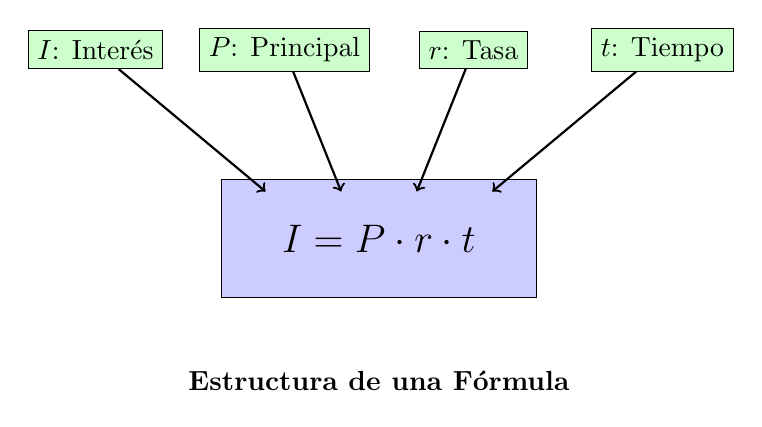
\begin{tikzpicture}[scale=1.2]
    % Central formula box
    \node[draw, fill=blue!20, minimum width=4cm, minimum height=1.5cm] (formula) at (0,0)
        {\Large $I = P \cdot r \cdot t$};

    % Variable explanations
    \node[draw, fill=green!20] (I) at (-3,2) {$I$: Interés};
    \node[draw, fill=green!20] (P) at (-1,2) {$P$: Principal};
    \node[draw, fill=green!20] (r) at (1,2) {$r$: Tasa};
    \node[draw, fill=green!20] (t) at (3,2) {$t$: Tiempo};

    % Arrows pointing to formula
    \draw[->, thick] (I) -- (-1.2,0.5);
    \draw[->, thick] (P) -- (-0.4,0.5);
    \draw[->, thick] (r) -- (0.4,0.5);
    \draw[->, thick] (t) -- (1.2,0.5);

    \node at (0,-1.5) {\textbf{Estructura de una Fórmula}};
\end{tikzpicture}
\end{center}

%========================================
% SECTION 3.7.1: Evaluación de Fórmulas
%========================================
\subsectiontitle{Evaluación de una Fórmula}

\begin{definition}
\textbf{Evaluar una fórmula} significa calcular el valor de una variable cuando conocemos los valores de las demás variables.
\end{definition}

\textbf{Regla importante:} Para evaluar una fórmula de $n$ variables, debemos conocer los valores de $(n-1)$ variables.

\begin{example}
\textbf{Ejemplo 1:} Evalúe la fórmula $I = Prt$ para $P = 500$, $r = 0.06$, $t = 4$.

\textbf{Solución:}
\begin{align}
I &= Prt\\
I &= 500 \cdot 0.06 \cdot 4\\
I &= 500 \cdot 0.24\\
I &= 120
\end{align}

Por tanto, el interés ganado es $\$120$.
\end{example}

\begin{example}
\textbf{Ejemplo 2:} Evalúe la fórmula $I = Prt$ para $I = 350$, $r = 0.06$, $t = 4$. Encuentre $P$.

\textbf{Solución:}
\begin{align}
I &= Prt\\
350 &= P \cdot 0.06 \cdot 4\\
350 &= P \cdot 0.24\\
P &= \frac{350}{0.24}\\
P &= 1458.33
\end{align}

Por tanto, el capital principal es aproximadamente $\$1458.33$.
\end{example}

%========================================
% SECTION 3.7.2: Despeje de Fórmulas
%========================================
\subsectiontitle{Procedimiento para Despejar una Variable en Fórmulas}

Frecuentemente es útil \textit{despejar} una fórmula para expresarla en términos de una variable específica.

\textbf{Procedimiento para despejar una variable:}
\begin{enumerate}
\item Identificar la variable que se desea despejar
\item Tratar las demás variables como si fueran constantes
\item Usar operaciones que producen ecuaciones equivalentes para aislar la variable deseada
\end{enumerate}

% Visual flowchart for solving formulas
\begin{center}
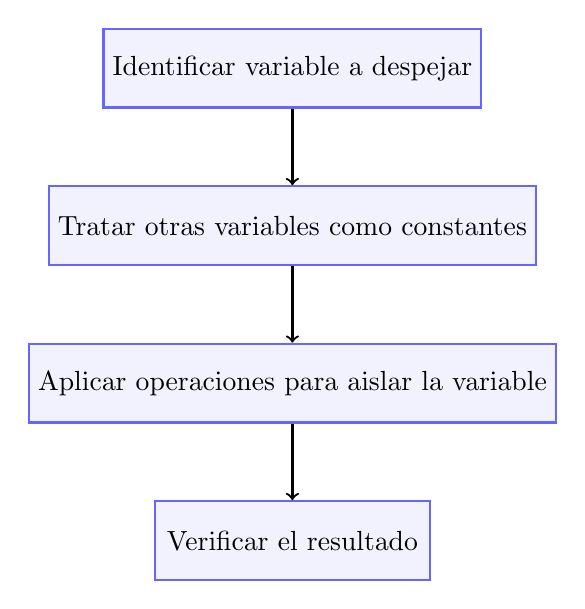
\begin{tikzpicture}[
    stepstyle/.style={rectangle, draw=blue!60, fill=blue!5, thick, minimum width=3.5cm, text centered, minimum height=1cm},
    arrowstyle/.style={->, thick}
]
    \node[stepstyle] (identify) at (0,0) {Identificar variable a despejar};
    \node[stepstyle] (treat) at (0,-2) {Tratar otras variables como constantes};
    \node[stepstyle] (isolate) at (0,-4) {Aplicar operaciones para aislar la variable};
    \node[stepstyle] (verify) at (0,-6) {Verificar el resultado};

    \draw[arrowstyle] (identify) -- (treat);
    \draw[arrowstyle] (treat) -- (isolate);
    \draw[arrowstyle] (isolate) -- (verify);
\end{tikzpicture}
\end{center}

\begin{example}
\textbf{Ejemplo 3:} Despeje la fórmula $I = Prt$ para la variable $t$.

\textbf{Solución:}
\begin{align}
I &= Prt\\
\frac{I}{Pr} &= \frac{Prt}{Pr} \quad \text{(dividir ambos lados por $Pr$)}\\
\frac{I}{Pr} &= t
\end{align}

Por tanto: $t = \frac{I}{Pr}$
\end{example}

\begin{example}
\textbf{Ejemplo 4:} Despeje la fórmula $I = Prt$ para la variable $r$.

\textbf{Solución:}
\begin{align}
I &= Prt\\
\frac{I}{Pt} &= \frac{Prt}{Pt} \quad \text{(dividir ambos lados por $Pt$)}\\
\frac{I}{Pt} &= r
\end{align}

Por tanto: $r = \frac{I}{Pt}$
\end{example}

%========================================
% SECTION 3.7.3: Fórmulas más Complejas
%========================================
\subsectiontitle{Fórmulas más Complejas}

\begin{example}
\textbf{Ejemplo 5:} Despeje la fórmula $A = P + Prt$ para la variable $t$.

\textbf{Solución:}
\textbf{Método 1 - Factorización:}
\begin{align}
A &= P + Prt\\
A &= P(1 + rt) \quad \text{(factorizar $P$)}\\
\frac{A}{P} &= 1 + rt \quad \text{(dividir por $P$)}\\
\frac{A}{P} - 1 &= rt \quad \text{(restar 1)}\\
\frac{\frac{A}{P} - 1}{r} &= t \quad \text{(dividir por $r$)}\\
t &= \frac{A - P}{Pr}
\end{align}

\textbf{Método 2 - Directo:}
\begin{align}
A &= P + Prt\\
A - P &= Prt \quad \text{(restar $P$)}\\
\frac{A - P}{Pr} &= t \quad \text{(dividir por $Pr$)}
\end{align}

Por tanto: $t = \frac{A - P}{Pr}$
\end{example}

\begin{example}
\textbf{Ejemplo 6:} Despeje la fórmula $A = P + Prt$ para la variable $P$.

\textbf{Solución:}
\begin{align}
A &= P + Prt\\
A &= P(1 + rt) \quad \text{(factorizar $P$)}\\
\frac{A}{1 + rt} &= P \quad \text{(dividir por $(1 + rt)$)}
\end{align}

Por tanto: $P = \frac{A}{1 + rt}$
\end{example}

\begin{example}
\textbf{Ejemplo 7:} Despeje la fórmula $C = \frac{5}{9}(F-32)$ para la variable $F$.

\textbf{Solución:}
\begin{align}
C &= \frac{5}{9}(F-32)\\
\frac{9C}{5} &= F - 32 \quad \text{(multiplicar por $\frac{9}{5}$)}\\
\frac{9C}{5} + 32 &= F \quad \text{(sumar 32)}
\end{align}

Por tanto: $F = \frac{9C}{5} + 32$
\end{example}

% Summary table of formulas and their variations
\begin{center}
\begin{tabular}{|c|c|c|}
\hline
\textbf{Fórmula Original} & \textbf{Variable Despejada} & \textbf{Fórmula Despejada} \\
\hline
$I = Prt$ & $P$ & $P = \frac{I}{rt}$ \\
\hline
$I = Prt$ & $r$ & $r = \frac{I}{Pt}$ \\
\hline
$I = Prt$ & $t$ & $t = \frac{I}{Pr}$ \\
\hline
$A = P + Prt$ & $P$ & $P = \frac{A}{1 + rt}$ \\
\hline
$A = P + Prt$ & $t$ & $t = \frac{A - P}{Pr}$ \\
\hline
$C = \frac{5}{9}(F-32)$ & $F$ & $F = \frac{9C}{5} + 32$ \\
\hline
\end{tabular}
\end{center}

\textbf{Nota importante:} El despeje de fórmulas utiliza los mismos principios que la resolución de ecuaciones lineales. La diferencia principal es que trabajamos con múltiples variables, tratando todas excepto la que despejamos como constantes.